\section{requirements engineering}\label{requirementsengineering}
Figure \ref{fig:useCaseDiagram} shows the use case diagram for ComeTogether.

\subsection{use cases}\label{usecases}

\textbf{UC 1.1 register - create profile}
\begin{enumerate}
\item start app
\item touch button "create profile"
\item input of personal data (name, gender, data of birth, email)
\item may upload a photo
\item input password
\item repeat password
\item touch button "register"
\end{enumerate}


\textbf{UC 1.2 login}
\begin{enumerate}
\item start app
\item user is automatically logged
\end{enumerate}


\textbf{UC 2.1 create event}
\begin{enumerate}
\item UC 1.2 login
\item touch "Offer" - Button
\item input data (date, place, titel) on the offer form
\item touch button "okay"
\item the generated event is added to the database and displayed on the search page
\end{enumerate}


\textbf{UC 2.2 search events}
\begin{enumerate}
\item UC 1.2 login
\item touch "search" - button
\item display all events in table form location based (via GPS in a 50km radius):
   	 � 3 categories (events, food \& beverage, sports- and leisure activities in table form):
\begin{enumerate}
\item date
\item place
\item title of event
\item number of participants and gender
\end{enumerate}
\begin{enumerate}
\item alternative scenario: input of specific date, any other place with different radius, category 
thru scrolling screen right
to automatically change and issuance of the new results, according to the data mentioned
\end{enumerate}
\item select desired event thru touch of a titel
\item display event description and with scrolling provider profil
\begin{enumerate}
\item alternative scenario 1: select an event thru touch of the "get in touch" button
\begin{enumerate}
\item open the mailbox with empty textbox and registered recipient or tenderer thru touch of the "get in touch" - button
\item writing a message and come into conatct with the provider thru sending the message
\item select number of participants and gender
\end{enumerate}
\item alternative sceanario 2: return to the overview thru back-button to select another event
\end{enumerate}
\end{enumerate}


\textbf{UC 2.3 delete event}
\begin{enumerate}
\item UC 1.2 login
\item touch "my events", to display a list of own events
\item select the own event in the list
\item delete event thru touch the delete button and the system generates automatically a denial mail for persons who already participate
\end{enumerate}


\textbf{UC 2.4 delete past events after a day}
\begin{enumerate}
\item past events are deleted automatically by the system after one day
\end{enumerate}


\textbf{UC 2.5 Event update / predict seekers}
\begin{enumerate}
\item UC 3.2 message recall
\item tenderer touches commitment button to update number of participants and their gender
\end{enumerate}


\textbf{UC 2.6 cancel an event}
\begin{enumerate}
\item UC 3.1 message recall
\item bidder touches cancel button, to generates automatically a denial mail for persons who already participate
\end{enumerate}


\textbf{UC 3.1 message recall}
\begin{enumerate}
\item UC 1.2 login
\item touch mailbox button
\item select message
\end{enumerate}


\textbf{UC 3.2 write message}
\begin{enumerate}
\item UC 3.1 message recall
\item touch reply button
\item write message
\item touch send button
\end{enumerate}


\textbf{UC 3.3 notify user if a new message arrives}
\begin{enumerate}
\item system sends automatically an email to the user
\end{enumerate}


\section{Design}\label{Design}

In figure \ref{fig:UserServiceREST} you can see the design for the UserService. UserServiceREST encapsulate the REST-Functionality of the UserService. UserPersistence access database with prepared statements p.e. to save, read or delete users. Between UserServiceREST and UserPersistence are service class and DAO class to encapsulate different levels of abstraction. Beside UserServiceREST there are the classes EventServiceREST, ParticipationServiceREST and MessageServiceREST. EventServiceREST in figure \ref{fig:EventServiceREST} creates, reads and deletes events. ParticipationServiceREST in figure \ref{fig:ParticipationServiceREST} creates participations and gives back a list of participation for a given eventid or a given userid. MessageServiceREST in figure \ref{fig:MessageServiceREST} creates, reads or deletes messages.

\begin{figure}[htp]
\centering
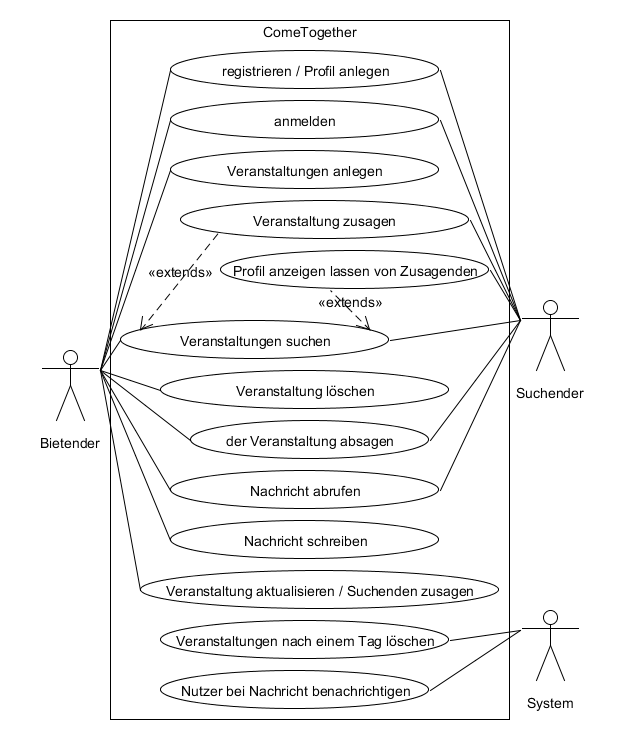
\includegraphics[width=0.5\textwidth]{Ingo/pictures/UseCaseDiagram.png}
\caption{use case diagram}
\label{fig:useCaseDiagram}
\end{figure}


\begin{figure}[htp]
\centering
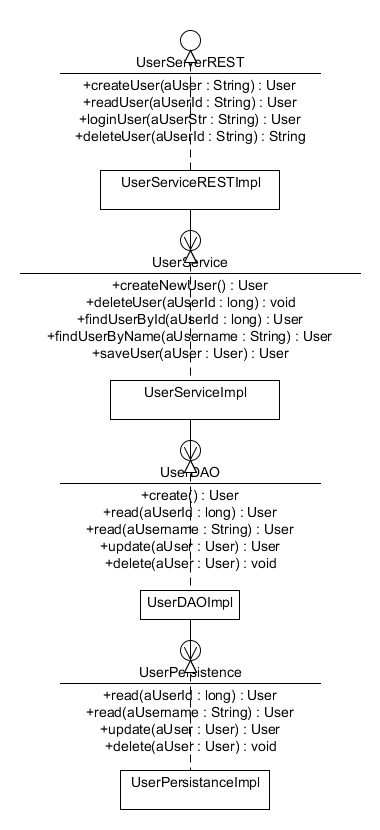
\includegraphics[width=0.5\textwidth]{Ingo/pictures/Design_User.png}
\caption{desing class diagramm UserServiceREST}
\label{fig:UserServiceREST}
\end{figure}


\begin{figure}[htp]
\centering
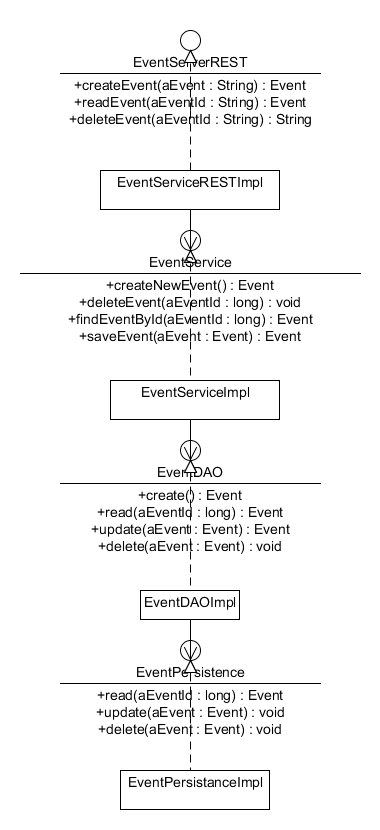
\includegraphics[width=0.5\textwidth]{Ingo/pictures/Design_Event.png}
\caption{desing class diagramm EventServiceREST}
\label{fig:EventServiceREST}
\end{figure}


\begin{figure}[htp]
\centering
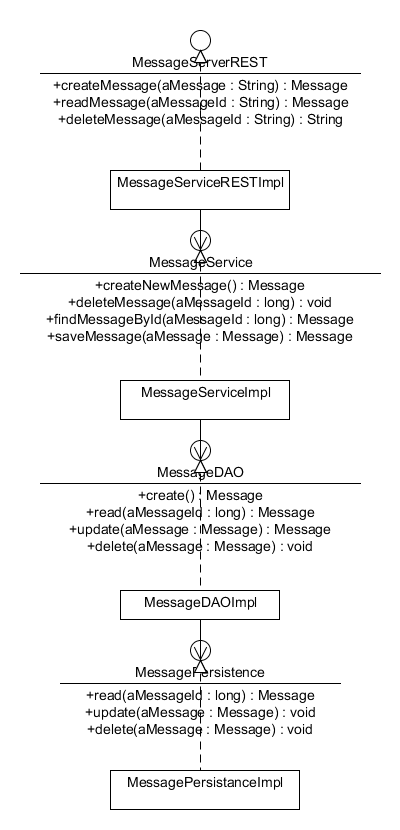
\includegraphics[width=0.5\textwidth]{Ingo/pictures/Design_Message.png}
\caption{desing class diagramm MessageServiceREST}
\label{fig:MessageServiceREST}
\end{figure}


\begin{figure}[htp]
\centering
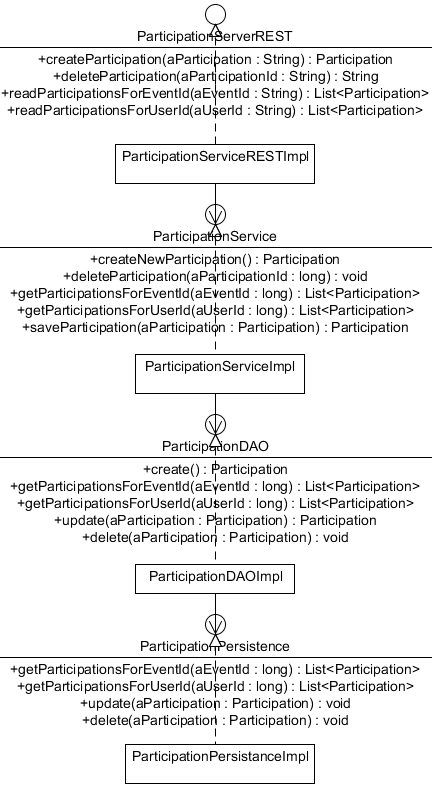
\includegraphics[width=0.5\textwidth]{Ingo/pictures/Design_Participation.png}
\caption{desing class diagramm ParticipationServiceREST}
\label{fig:ParticipationServiceREST}
\end{figure}
